%Teilauswertung Brewster

\section{Bestimmung des Verstärkungsfaktors}
\subsection{Brewster- und Grenzwinkel}

Bei der Aufnahme des Intensitätsplots übersteuerte die Diode teilweise, 
weshalb Abb.\ref{plot:Talpha}, in dem die transmittierte Intensität in relativen Einheiten gegen den Einfallswinkel aufgetragen ist, nicht den vollständigen Verlauf zeigt, 
da der Graph bei der relativen Einheit 1 abgeschnitten ist. 
%Der Verlauf des Transmissionskoeffizienten $T = \frac{I_T}{I_0}$ aufgetragen gegen den Winkel des Glasplättchens ist in Abb.\ref{plot:Talpha} gezeigt.

\begin{figure}[h]
    \centering
    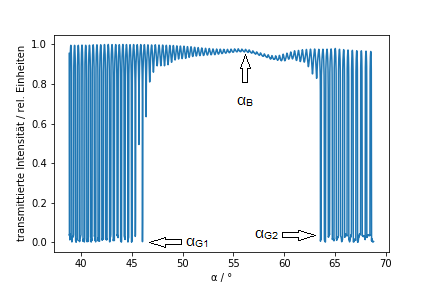
\includegraphics[scale = 1.5]{Bilder/Auswertung/brewsterpfeil.png}
    \caption{Der Winkel des in den Resonator eingebrachten Glasplättchens $\alpha$ wird von 60°-90° in 0,01°-Schritten variiert. Aufgetragen ist die transmittierte Intensität 
    des Lasers in relativen Einheiten gegen $\alpha$ in Grad. Dabei übersteuerte die verwendete Photodiode regelmäßig. Auffällig ist der oszillierende Verlauf. 
    Zudem sind die Grenzwinkel $\alpha_G$ und der Brewsterwinkel $\alpha_B$ eingezeichnet.}
    \label{plot:Talpha}
\end{figure}

Im Graphen ist zunächst einmal der oszillierende Verlauf des Transmissionskoeffizienten auffällig. Dies lässt sich durch die Airy-Formel für die transmittierte Intensität 
erklären. Sie lautet 
\begin{equation}
    I_T = I_0 \frac{1}{1+F \sin^2(\frac{\Delta \phi}{2})}  
    \label{eq:airy}
\end{equation}
mit den Abkürzungen 
\begin{equation}
    F = \frac{4R}{(1-R)^2} \quad \mathrm{ und } \quad \Delta \phi = \frac{4\pi}{\lambda}d\sqrt{n^2-\sin^2\alpha},
    \label{eq:airyPar}
\end{equation} 
wobei $R$ der Reflektionskoeffizient ist.\\
In Gl.\ref{eq:airy} ist zu sehen, dass das $I_T = I_0$ für $\sin^2(\frac{\Delta \phi}{2}) = 0$ gilt. Da $\Delta \phi$ wiederum von $\sin^2\alpha$ abhängt, oszilliert auch die 
transmittierte Intensität.\\
Der Brewsterwinkel $\alpha_B$ ist derjenige Winkel, bei dem zur Einfallsebene parallel polarisiertes Licht vollständig transmittiert wird. Folglich erwarten wir $\alpha_B$ 
im absoluten Maximum in Abb.\ref{plot:Talpha}. Da die Photodiode aber regelmäßig übersteuerte, ist diese Identifizierung in diesem Fall nicht möglich. Stattdessen können wir 
aber einfach das maximale Minimum der transmittierten Intensität auslesen und im Fehlerbereich die benachbarten Maxima einschließen. Somit ergibt sich ein Brewsterwinkel von 
\begin{equation*}
    \textcolor{red}{\alpha_B = (55,7 \pm 0,2)^\circ}.
\end{equation*}
Die Grenzwinkel $\alpha_G$ sind definiert als die Winkel, bei denen der Laser erstmals anspringt bzw. erlischt, die transmittierte Intensität also auf 0 abfällt. Diese lesen sich 
ab zu 
\begin{equation*}
    \textcolor{red}{\alpha_{G1} = (46,05 \pm 0,05)^\circ \quad} \mathrm{ und } \textcolor{red}{ \quad \alpha_{G2} = (63,60 \pm 0,05)^\circ}.
\end{equation*}
Der Brewsterwinkel ist verknüpft mit dem Brechungsindex über die Beziehung 
\begin{equation*}
    \tan\alpha_B = \frac{n_2}{n_1}.
\end{equation*}
Für $n_1 = 1$ (Luft) folgt der Brechungsindex des Glasplättchens mit Fehlerfortpflanzung zu 
\begin{equation*}
    \textcolor{red}{n_{Glas} = 1,466 \pm 0,011},
\end{equation*}
was im Bereich des Brechungsindex von Glas liegt.\footnote{\url{https://www.edmundoptics.de/knowledge-center/application-notes/optics/optical-glass/}, Stand: 11.10.21} 
Demnach kann unser Ergebnis für $\alpha_B$ als sinnvoll angesehen werden.
$\alpha_B$ und die $\alpha_G$ sind auch in Abb.\ref{plot:Talpha} eingezeichnet. Dabei ist eine leichte Asymmetrie des Graphen bezüglich $\alpha_B$ zu erkennen. Gl.\ref{eq:airy} ist zwar auf den 
ersten Blick symmetrisch, doch betrachtet man das darin vorkommende $F$ in Gl.\ref{eq:airyPar} genauer, so stellt man eine Abhängigkeit vom Reflektiosnkoeffizienten $R$ fest. 
Dieser ist über die Fresnel'schen Formeln definiert als 
\begin{equation*}
    R =\biggl (\frac{E_{0r}}{E_{0e}} \biggl)^2 = \biggl(\frac{n_2\cos\alpha - \cos\beta}{n_2\cos\alpha + \cos\beta} \biggl)^2 = \biggl(\frac{n_2^3\cos\alpha - (n_2^2-\sin^2\alpha)}{n_2^3\cos\alpha - (n_2^2-\sin^2\alpha)} \biggl)^2,
\end{equation*}
wobei $n_1 = 1$ angenommen wurde. In dieser Gleichung ist zu sehen, dass der Reflektionskoeffizient $R$ wiederum von $\alpha$ abhängt. Trägt man diese nun gegeneinander auf, so ist zu erkennen, dass keine 
Symmetrie bezüglich $\alpha_B$ existiert (\cite{Demtroeder2017}, S.224). Deshalb ist auch im Graphen der transmittierten Intensität eine solche Asymmetrie zu sehen.


\subsection{Verstärkungsfaktor}
Um den Verstärkungsfaktor des laseraktiven Mediums zu berechnen, ist es sinnvoll zunächst einmal die Gewinn-Verlust-Bilanz bei einem Durchlauf im Resonator aufzustellen. 
Dazu betrachte man Abb.\ref{pic:SchemaBrew}, die aus dem Versuchsskript entnommen wurde.
\begin{figure}[h]
    \centering
    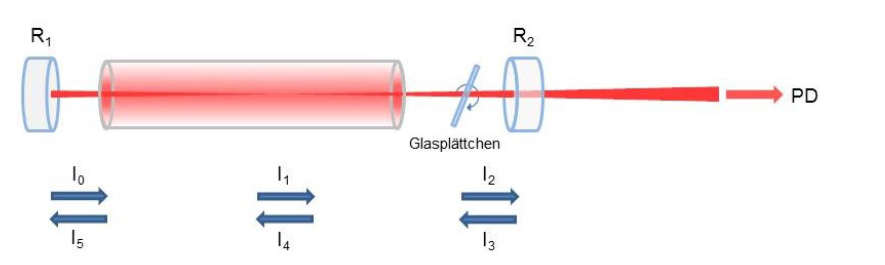
\includegraphics[scale = 0.5]{Bilder/Auswertung/SchemaBrew.png}
    \caption{Schematischer Durchlauf durch den Resonator mit eingebautem Glasplättchen; aus dem Versuchsskript entnommen.}
    \label{pic:SchemaBrew}
\end{figure}
Im Resonator berechnet sich die Intensität $I_6$ nach einem Durchlauf (die in Abb.\ref{pic:SchemaBrew} äquivalent zu $I_0$ liegt) wie folgt:
\begin{align*}
    I_6 &= R_1 I_5 = \\
    &= R_1 v I_4 = \\
    &= R_1 v T I_3 = \\
    &= R_1 v T R_2 I_2 = \\
    &= R_1 v T^2 R_2 I_1 = \\
    &= R_1 v^2 T^2 R_2 I_0\\
\end{align*}
Hierbei sind $R_{1/2}$ die Reflektiosnkoeffizienten der Spiegel 1 bzw. 2 und $T$ der Transmissionskoeffizient des Glasplättchens. Im Bereich der Grenzwinkel ist die 
Gewinn-Verlsut-Billanz ausgeglichen, der Resonator ist im Leerlaufmodus ($I_0 \rightarrow 0$). Mit der Bedingung $I_0 = I_6$ folgt für den Verstärkungsfaktor 
\begin{equation*}
    v = \frac{1}{\sqrt{R_1R_2}T}.
\end{equation*}
Nimmt man die Strahlung durch das Glasplättchen als verlustfrei an, so gilt $T = 1-R$ und über die Fresnell'sche Formel
\begin{equation*}
    R = \frac{\tan(\alpha - \beta)}{\tan(\alpha + \beta)}
\end{equation*}
folgen mit dem Snellius'schen Brechungsgesetz
\begin{equation*}
    \beta = \arcsin(\frac{\sin\alpha}{n_{Glas}})
\end{equation*}
die Verstärkungsfaktoren für $\alpha_{G1}$ und $\alpha_{G2}$ zu 
\begin{equation*}
    v_1 = 1,01676 \pm 0,00014 \quad \mathrm{ und } \quad v_2 = 1,0202 \pm 0,0036,
\end{equation*}
wobei folgende Beziehungen für die Fehlerrechnung verwendet wurden:
\begin{align*}
    s_v &= \frac{s_R}{\sqrt{R_1R_2}(1-R)^2}\\
    s_R &= \sqrt{(\partial_\alpha R s_\alpha)^2 + (\partial_nRs_n)^2}\\
    \partial_\alpha R &= \frac{\frac{(1-\frac{\cos\alpha}{\sqrt{n^2-\sin^2\alpha}})\tan(\alpha+\arcsin(\frac{\sin\alpha}{n}))} {\cos^2(\alpha-\arcsin(\frac{\sin\alpha}{n}))} - \frac{(1+\frac{\cos\alpha}{\sqrt{n^2-\sin^2\alpha}})\tan(\alpha-\arcsin(\frac{\sin\alpha}{n}))} {\cos^2(\alpha+\arcsin(\frac{\sin\alpha}{n}))}} {\tan^2(\alpha - \arcsin(\frac{\sin\alpha}{n}))}\\
    \partial_nR &= \frac{\sin\alpha(\frac{\tan(\alpha+\arcsin(\frac{\sin\alpha}{n}))}{\cos^2(\alpha-\arcsin(\frac{\sin\alpha}{n}))} - \frac{\tan(\alpha-\arcsin(\frac{\sin\alpha}{n}))}{\cos^2(\alpha+\arcsin(\frac{\sin\alpha}{n}))})}{\tan^2(\alpha + \arcsin(\frac{\sin\alpha}{n}))}\\
\end{align*}
Mittelt man über beide Verstärkungsfaktoren, so erhält man einen Verstärkungsfaktor von 
\begin{equation*}
    \textcolor{red}{v = 1,0185 \pm 0,0018}.
\end{equation*}
Dies entspricht den Erwartungen, dass im Leerlauf der Verstärkungsfaktor ungefähr 1 ist.\\
Verwendet man nun nicht die Näherung, dass das Glas absorptionsfrei ist, so berechnet sich $T$ über die Airy-Formel zu 
\begin{equation*}
    T = \frac{1}{1+F\sin^2(\frac{2\pi d}{\lambda}\sqrt{n^2-\sin^2\alpha})}
\end{equation*}
mit den Abkürzungen aus Gl.\ref{eq:airyPar}.\\
Kennt man nun die Dicke $d$ und nimmt den Winkel $\alpha$ als gegeben an, kann man den Fehler von o.B.d.A. $v_1$ wie folgt berechnen ($v_2$ funktioniert analog und liefert keinen Mehrwert):
\begin{equation*}
    s_{v_1} = \sqrt{(\partial_dvs_d)^2 + (\partial_nvs_n)^2},
\end{equation*}
wobei sich die partiellen Ableitungen ergeben zu:
\begin{align*}
    \partial_dv &= \frac{F}{\sqrt{R_1R_2}}\sin(\frac{4\pi d}{\lambda}\sqrt{n^2-sin^2\alpha})\frac{2\pi}{\lambda}\sqrt{n^2-\sin^2\alpha}\\
    \partial_nv &= \frac{1}{\sqrt{R_1R_2}} \Bigg[ F \sin(\frac{4\pi d}{\lambda}\sqrt{n^2-sin^2\alpha})\frac{2nd\pi}{\lambda \sqrt{n^2-\sin^2\alpha}}\\
    &+ \sin^2\biggl(\frac{2\pi d}{\lambda}\sqrt{n^2-sin^2\alpha} \biggl ) \frac{4(1-R)^2+8(1-R)R}{(1-R)^4} \frac{\sin\alpha}{n\sqrt{n^2-\sin^2\alpha}\tan^2(\alpha+ \arcsin(\frac{\sin\alpha}{n}))}\\
    &\cdot \biggl (\frac{\tan(\alpha - \arcsin(\frac{\sin\alpha}{n}))}{\cos^2(\alpha + \arcsin(\frac{\sin\alpha}{n}))} - \frac{\tan(\alpha+ \arcsin(\frac{\sin\alpha}{n}))}{\cos^2(\alpha - \arcsin(\frac{\sin\alpha}{n}))} \biggl ) \Bigg]
\end{align*}
Ziel ist es, den Fehler für die Dicke des Plättchens $s_d$ so zu bestimmen, dass die selbe Ungenauigkeit wie bei der Drehspiegelmethode erzielt wird. Aus der Gleichsetzung der 
Fehler $s_{v_1}$ folgt dann 
\begin{equation*}
    s_d = \sqrt{s_{v_1}^2 - (\partial_nvs_n)^2}(\partial_dv)^{-1}.
\end{equation*}
Für $d = 250\,\mu$m (aus Versuchsskript), $\lambda = 632,8\,$nm und den bisher berechneten Werten 
kommt es zu keinem sinnvollen Ergebnis, da schon alleine der Fehleranteil des Brechungsindices bei der Bestimmung über die Plättchendicke größer ist als der 
Gesamtfehler der Drehspiegelmethode. Nimmt man nun auch $n$ als fehlerfrei an, so ergibt sich 
\begin{equation*}
    s_d = \frac{s_{v_1}}{\partial_dv} = 0,81 \mathrm{nm},
\end{equation*}
was ein sehr niedriger Wert ist, der mit einfachen Messmethoden nicht zu erreichen ist. Demnach ist entweder der Vergleich der Fehler selbst fehlerhaft oder die Drehspiegelmethode 
liefert wesentlich präzisere Ergebnisse.\\
Die Plättchendicke lässt sich über die Interferenzbedingung zusammen mit Gl.\ref{eq:airyPar} bestimmen:
\begin{equation}
    \Delta \phi = \frac{4\pi}{\lambda}d\sqrt{n^2-\sin^2\alpha} \overset{!}{=} 2\pi m 
    \label{eq:intbed}
\end{equation}
Hierbei ist $m$ eine ganze Zahl. Liest man nun die Maxima bei $m$ und $m+i$ aus, so ergibt sich $d$ aus Gl.\ref{eq:intbed} zu 
\begin{equation*}
    d = \frac{i\lambda}{2(\sqrt{n^2-\sin^2\alpha_{m+i}} - \sqrt{n^2-\sin^2\alpha_m})}.
\end{equation*}
Mit $\alpha_m = (39,0 \pm 0,1)^\circ$ und $\alpha_{m+79} = (68,55 \pm 0,05)^\circ$ folgt 
\begin{equation*}
    \textcolor{red}{d = (130,6 \pm 1,5)\,\mu\mathrm{m}}.
\end{equation*}
Für die Fehlerrechnung wurden folgende partielle Ableitungen verwendet:
\begin{align*}
    \partial_nd &= \frac{-in\lambda}{2}\big(\sqrt{n^2-\sin^2\alpha_{m+i}}- \sqrt{n^2-\sin^2\alpha_{m}}\big)^{-2}\big(\frac{1}{n^2-\sin^2\alpha_{m+i}} - \frac{1}{n^2-\sin^2\alpha_{m}}\big)\\
    \partial_{\alpha_{m/m+i}}d &= \frac{i\lambda}{2}\big(\sqrt{n^2-\sin^2\alpha_{m+i}}- \sqrt{n^2-\sin^2\alpha_{m}}\big)^{-2}\bigg(\frac{\mp \sin(2\alpha_{m/m+i})}{2\sqrt{n^2-\sin^2\alpha_{m/m+i}}}\bigg)\\
\end{align*}
Die Dicke stimmt in der Größenordnung mit der Angabe von 150\,$\mu$m im Versuchsskript überein, jedoch nicht innerhalb des berechneten Fehlers. Entweder wurde dieser zu klein 
abgeschätzt oder, was unserer Meinung nach wahrscheinlicher ist, in der Angabe im Skript ist im Wort 'circa' eine größere Abweichung enthalten.